\documentclass[12pt]{extarticle}
%Some packages I commonly use.
\usepackage[english]{babel}
\usepackage{graphicx, wrapfig}
\usepackage{framed}
\usepackage[normalem]{ulem}
\usepackage{amsmath}
\usepackage{amsthm}
\usepackage{amssymb}
\usepackage{amsfonts}
\usepackage{enumerate}

\usepackage{hyperref}

\usepackage[utf8]{inputenc}
\usepackage[top=1 in,bottom=1in, left=1 in, right=1 in]{geometry}

%A bunch of definitions that make my life easier
\newcommand{\matlab}{{\sc Matlab} }
\newcommand{\cvec}[1]{{\mathbf #1}}
\newcommand{\rvec}[1]{\vec{\mathbf #1}}
\newcommand{\ihat}{\hat{\textbf{\i}}}
\newcommand{\jhat}{\hat{\textbf{\j}}}
\newcommand{\khat}{\hat{\textbf{k}}}
\newcommand{\minor}{{\rm minor}}
\newcommand{\trace}{{\rm trace}}
\newcommand{\spn}{{\rm Span}}
\newcommand{\rem}{{\rm rem}}
\newcommand{\ran}{{\rm range}}
\newcommand{\range}{{\rm range}}
\newcommand{\mdiv}{{\rm div}}
\newcommand{\proj}{{\rm proj}}
\newcommand{\R}{\mathbb{R}}
\newcommand{\N}{\mathbb{N}}
\newcommand{\Q}{\mathbb{Q}}
\newcommand{\Z}{\mathbb{Z}}
\newcommand{\<}{\langle}
\renewcommand{\>}{\rangle}
\renewcommand{\emptyset}{\varnothing}
\newcommand{\attn}[1]{\textbf{#1}}
\theoremstyle{definition}
\newtheorem{theorem}{Theorem}
\newtheorem{corollary}{Corollary}
\newtheorem*{definition}{Definition}
\newtheorem*{example}{Example}
\newtheorem*{note}{Note}
\newtheorem{exercise}{Exercise}
\newcommand{\bproof}{\bigskip {\bf Proof. }}
\newcommand{\eproof}{\hfill\qedsymbol}
\newcommand{\Disp}{\displaystyle}
\newcommand{\qe}{\hfill\(\bigtriangledown\)}
\setlength{\columnseprule}{1 pt}


\title{BMIF 201 Lecture 3}
\author{Michelle M. Li}
\date{September 11, 2019}

\begin{document}

\maketitle

\section{Review: Taylor's Expansion}

\textbf{Motivation:} Calculating values (i.e. $e^x$) is difficult for humans (and often even computers)\\

\noindent \textbf{Example:} Suppose our function is $sin(x)$ and we want to calculate the value of the red dot in Figure \ref{fig1}. If $X$ is large, it is very difficult to compute the exact value. Instead, we can use Taylor's Expansion to approximate the purple function in Figure \ref{fig1}.

\begin{figure}[h]
\caption{Approximating $\sin (x)$}
\centering
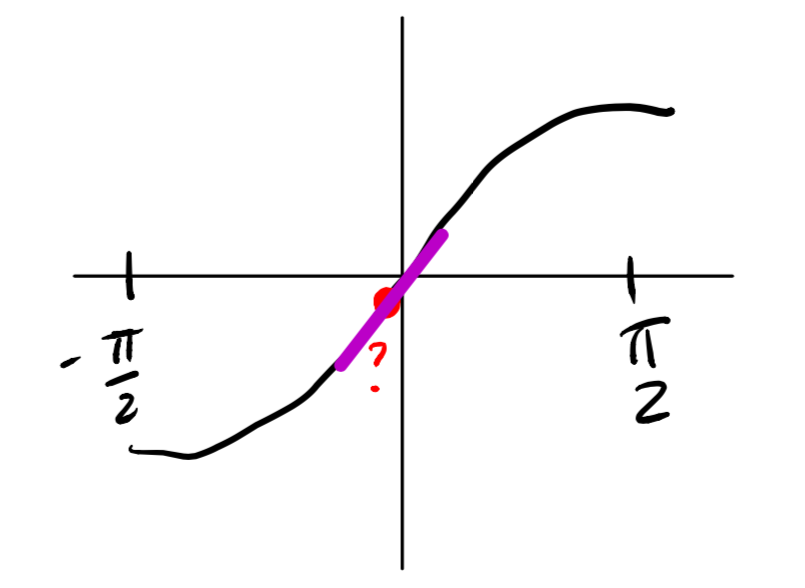
\includegraphics[width=0.3\textwidth]{fig1.png}
\label{fig1}
\end{figure}


\noindent Let
\begin{equation}
    T(X) = a_0 + a_1 x + a_2 x^2 + a_3 x^3
\end{equation}
and set $a_0$, $a_1$, $a_2$, and $a_3$ such that
\begin{align*}
    T(0) &= sin(0)\\
    T'(0) &= sin'(0)\\
    T''(0) &= sin''(0)\\
    T'''(0) &= sin'''(0)
\end{align*}
So, for $T(X)$,
\begin{align*}
    T(X) &= a_0 + a_1 x + a_2 x^2 + a_3 x^3\\
    T'(X) &= a_1 + 2a_2 x + 3a_3 x^2\\
    T''(X) &= 2a_2 + 3*2a_3 x\\
    T'''(X) &= 3*2a_3
\end{align*}
and
\begin{align*}
    sin(x) &= 0\\
    sin'(x) = cos(x) &= 1\\
    sin''(x) = -sin(x) &= 0\\
    sin'''(x) = -cos(x) &= -1
\end{align*}
Hence, at $X = 0$,
\begin{align*}
    T(0) &= a_0 = 0\\
    T'(0) &= a_1 = 1!a_1 = 1\\
    T''(0) &= 2a_2 = 2!a_2 = 0\\
    T'''(0) &= 3*2a_2 = 3!a_3 = -1
\end{align*}
Finally, we derive the Taylor's Expansion as
\begin{equation}
    f(x) = \sum_{k = 0}^n \frac{f^{(k)}(a)}{k!}(x - a)^k \label{taylor}
\end{equation}
Expanding (\ref{taylor}), we get
\begin{equation}
    f(x_1, \dots, x_d) = \sum_{i_1 = 0}^m \dots \sum_{i_d = 0}^m \frac{\partial^{i_1} \dots \partial^{i_d}}{i_1!\dots i_d! \partial_{x_1}^{i_1}\dots \partial_{x_d}^{i_d}} f(a_1, \dots, a_d)(x_1 - a_1)^{i_1}\dots(x_d - a_d)^{i_d}
\end{equation}
Using an example, where $m = 2$,
\begin{equation}
    f(x, y) = e^x \ln(1 + y) \approx y + xy - y^2
\end{equation}
Here is how we arrived at that approximation. The derivatives are as follows
\begin{align}
    \frac{\partial f}{\partial x} &= e^x \ln(1 + y)\\
    \frac{\partial^2 f}{\partial^2 x} &= e^x \ln(1 + y)\\
    \frac{\partial f}{\partial y} &= \frac{e^x}{1 + y}\\
    \frac{\partial^2 f}{\partial^2 x} &= e^x \left( -\frac{1}{(1 + y)^2}\right)\\
    \frac{\partial f}{\partial x \partial y} &= \frac{e^x}{1 + y}\\
\end{align}
At $(x, y) = 0$, 
\begin{align}
    \frac{\partial f}{\partial x} &= 0\\
    \frac{\partial^2 f}{\partial^2 x} &= 0\\
    \frac{\partial f}{\partial y} &= 1\\
    \frac{\partial^2 f}{\partial^2 x} &= -1\\
    \frac{\partial f}{\partial x \partial y} &= 1\\
\end{align}
\textbf{Notes:}
\begin{itemize}
    \item $\frac{\partial^2 f}{\partial x \partial y} \neq \frac{\partial^2 f}{\partial x \partial y}$ depending on the function.
\end{itemize}

\section{Heterozygosity Equation}

\textbf{Recall:} CZ posed the question, ``Why does the Moran and Wright-Fisher models fixate when the heterozygosity equation (1) suggests otherwise?"
\begin{align}
    H_t &= H_0(1 - \frac{1}{N})^t \nonumber \\
    &\approx H_0e^{-\frac{t}{N}} \label{H_0}
\end{align}

\noindent For some time $t$, the expected heterozygosity for two alleles is as follows
\begin{align}
    H_{t + 1} &= \frac{1}{N}*0 + (1 - \frac{1}{N})*H_t \nonumber \\
    &= (1 - \frac{1}{N})*H_t \label{H_t}
\end{align}
where $\frac{1}{N}$ is the probability two offspring share the same ancestor, and $(1 - \frac{1}{N})$ is the probability that they do not.\\

\noindent \textbf{Explanation:} We are calculating the expected value of the next time step. The probability of reaching, thereby fixating at, $0$ or $N$ is non-zero.

\section{Wright-Fisher Model}

\subsection{Background}

In the Wright-Fisher Model (a.k.a. Fisher-Wright Model), you choose $n$ alleles (white or black) from the population of a set size $N$.\\

\noindent The probability of choosing a black allele is $p = \frac{b}{N}$, where $b$ is the number of black alleles in the population at time $t$.\\

\noindent This is a binomial distribution problem, where you are doing $n$ ``coin flips" of probability $p$ to get the number of black alleles, $X$.
\begin{equation}
    X \sim Bin(n, p) \label{bin}
\end{equation}

\subsection{Simulations}
Simulation exercises can be found here as a Jupyter Notebook: \url{https://github.com/michellemli/BMIF201}\\

\subsection{Shannon Entropy}

The class seems to agree that the time to fixation when $N = 20$ and $p = 0.5$ is around 27. We will now derive the results.\\

\noindent Firstly, the Shannon entropy is defined as
\begin{equation}
    S(X) = -\sum p_i \log_i(p_i) \label{S_X}
\end{equation}
where $\displaystyle p_i = \frac{x_i}{N}$. When $p = 0.5$, the entropy is at its peak (Figure \ref{fig2}).

\begin{figure}[h]
\caption{Shannon Entropy}
\centering
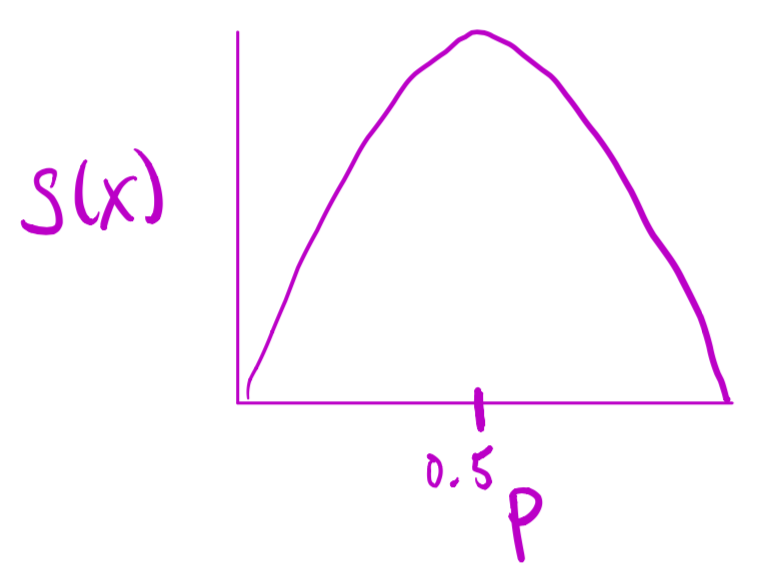
\includegraphics[width=0.3\textwidth]{fig2.png}
\label{fig2}
\end{figure}

\noindent At fixation, this value is $0$ because there is only one allele in the population.
\begin{equation}
    S(X) = 0 \Longleftrightarrow \text{Fixation} \nonumber
\end{equation}
The partial derivatives of $S(X)$ are
\begin{align}
    \frac{\partial S(X)}{x_i} &= -\frac{1}{N}(1 + \log(\frac{x_i}{N})) \nonumber \\
    \frac{\partial^2 S(X)}{\partial x_i \partial x_j} &= -\frac{\delta_{ij}}{Nx_j} \label{partial^2}
\end{align}
where
\begin{equation}
    \delta_{ij} = \begin{cases}
        1, & \text{if } i = j\\
        0, & \text{if } i \neq j
    \end{cases} \label{delta}
\end{equation}
Recall that the expectation for selecting $j$ alleles with probability $p$ is
\begin{align}
    \left< j \right> &= np \label{exp}
\end{align}
and the variance is
\begin{align}
    Var \left< j \right> &= \left< j^2 \right> - \left< j \right>^2 \label{var1} \\
    &= np(1-p) \label{var2}
\end{align}
because the Wright-Fisher Model follows a binomial distribution.\\

\noindent To calculate the change in Shanon entropy over one time step:

\noindent Let $k$ be the number of alleles, and $x$ be the number of black alleles.
\begin{align}
    \left< S(x + \Delta x) \right> &\approx  \left<S(x) + \sum_i^k \frac{\partial S(x)}{\partial x}\Delta x_i + \frac{1}{2}\sum_i^k \sum_i^k \frac{\partial^2 S(x)}{\partial x_i \partial x_j} \right> \label{S1} \\
    &= S(x) + \sum_i^k \frac{\partial S(x)}{\partial x_i} \left< \Delta x_i \right> + \frac{1}{2}\sum_i^k \sum_j^k \frac{\partial^2 S(x)}{\partial^2 x_i \partial^2 x_j} \left< \Delta x_i \Delta x_j \right> \label{S2} \\
    &= S(x) + \frac{1}{2}\sum_i^k \sum_j^k \frac{\partial^2 S(x)}{\partial^2 x_i \partial^2 x_j} \left< \Delta x_i \Delta x_j \right> \label{S3} \\
    &= S(x) - \frac{1}{2}\sum_i^k \sum_j^k \frac{\delta_{ij}}{Nx_j} \left< \Delta x_i \Delta x_j \right> \label{S4} \\
    &= S(x) - \frac{1}{2}\sum_i^k \frac{1}{Nx_i} \left< \Delta x_i \Delta x_i \right> \label{S5} \\
    &= S(x) - \frac{1}{2}\sum_i^k \frac{1}{Nx_i} \left(N(\frac{x_i}{N})(1 - \frac{x_i}{N})\right) \label{S6} \\
    &= S(x) - \frac{1}{2N}\sum_i^k(1 - \frac{x_i}{N}) \label{S7} \\
    &= S(x) - \frac{k - 1}{2N} \label{S8}
\end{align}

\noindent \textbf{Remarks:}
\begin{itemize}
    \item Taking the partial derivative of $x_i$ in (\ref{S2}) results in $\left< \Delta x_i \right> = 0$.
    \item For (\ref{S3}), substitute with (\ref{partial^2}) to get (\ref{S4}).
    \item For (\ref{S4}), recall that $\delta_{ij} = 1$ when $i = j$ from (\ref{delta}).
    \item For (\ref{S5}), apply the variance equation (\ref{var2}) where $p = \frac{x_i}{N}$ to get (\ref{S6}).
    \item For (\ref{S6}), pull out the $N$ from the summation to get (\ref{S7}).
    \item For (\ref{S7}), remember that $\sum_i^k 1 = k$ and $\sum_i^k x_i = N$, which simplifies (\ref{S7}) into (\ref{S8}).
\end{itemize}

\noindent So, the expected change in Shannon entropy from generation to generation is
\begin{align}
    \left< \Delta S(X) \right> &= \left< S(x + \Delta x) \right> - S(x) = -\frac{k - 1}{2N} \label{ES}
\end{align}
To calculate the fixation time $T$, we start by stating that
\begin{align}
    S(X) - T \left< \Delta S(X) \right> = 0 \nonumber
\end{align}
where, after substituting in (\ref{ES}),
\begin{align}
    T &= \frac{S(X)}{\left< \Delta S(X) \right>} = \frac{2NS(X)}{k - 1} \nonumber
\end{align}

\end{document}

